% Robustness to rewiring (Sec. sec:robust of the main text)

The robustness sweep extends the rewiring of every ring setting to $p=0,0.01,\dots,1$
on the ten test graphs (seeds $0$--$9$), OSLOM and the stochastic block model in steps
of $0.05$; every other setting of the benchmarks is unchanged
(\texttt{bench/run2.py} with \texttt{DENSE\_P=1}; analysis in
\texttt{analysis/robust\_dense.py}). For each method and protocol, $p_{0.6}$ is the
first $p$ at which the mean $\Omega$ over the ten graphs falls below $0.6$, by linear
interpolation between grid points, and the area is the mean $\Omega$ over
$p\in[0,1]$. The planted-structure markers are computed on the same graphs: a ring is a
weak community when its members have more edges inside it than out, and $p_{\rm weak}$
is the first $p$ at which fewer than half of the rings are; $p_{\rm clust}$ is the first
$p$ at which the mean clustering coefficient is below $5\%$ of its value at $p=0$.

Table~\ref{tab:S-robust} gives, for every setting, HyperCommon's $p_{0.6}$ against the
other method that holds longest, with a paired bootstrap interval (\texttt{analysis/robust\_table.py});
the same comparison at the levels $0.5,0.7,0.8,0.9$ and by area is in
\texttt{figures/data/robust\_drop.csv}. \tbd{OSLOM and the SBM: complete on the uniform
and the first heterogeneous sweep; on the others still running.}

\begin{table*}[p]
\caption{Robustness to rewiring on the 28 ring settings: $p_{0.6}$, the rewired fraction at which the mean $\Omega$ over the ten test graphs first falls below $0.6$ (linearly interpolated between grid points), for HyperCommon (HC) and for the other method that holds longest, HC's rank among the seventeen methods and HC minus the best other method, with the paired 95\% bootstrap interval of HC minus the best of all other methods (the test graphs resampled, every mean curve recomputed and the best other method chosen again in each resample); the areas under the curves, with the same intervals, are in \texttt{figures/data/robust\_table.csv}. Label-free: every parameter by the largest overlapping modularity; oracle: the best parameter per graph. $p_{\rm weak}$, $p_{\rm clust}$: the planted-structure markers of Sec.~\ref{sec:robust}; $p_{\rm clust}>1$: the clustering never falls below $5\%$ of its value at $p=0$. Rewiring is uniform except where marked preferential (pref.) with exponent $\alpha$.}
\label{tab:S-robust}
\scriptsize\setlength{\tabcolsep}{2pt}
\begin{ruledtabular}
\begin{tabular}{llcc|cl r c|cl r c}
 & & & & \multicolumn{4}{c|}{label-free} & \multicolumn{4}{c}{oracle} \\
Setting & $o_n$ & $p_{\rm weak}$ & $p_{\rm clust}$ & HC & best other & rank & HC $-$ best & HC & best other & rank & HC $-$ best \\
\hline
uniform, $k=8$ & 0 & 0.51 & 0.65 & 0.46 & L-CPM 0.45 & 1 & $+0.00$ [$-0.00,+0.01$] & 0.46 & Leiden 0.49 & 3 & $-0.04$ [$-0.04,-0.03$] \\
uniform, $k=8$ & 0.05 & 0.47 & 0.65 & 0.36 & Leiden 0.36 & 2 & $-0.00$ [$-0.03,+0.02$] & 0.42 & Link 0.42 & 1 & $+0.01$ [$-0.00,+0.01$] \\
uniform, $k=8$ & 0.10 & 0.42 & 0.65 & 0.34 & Ego 0.35 & 2 & $-0.00$ [$-0.01,+0.01$] & 0.37 & Link 0.38 & 2 & $-0.00$ [$-0.02,+0.01$] \\
uniform, $k=16$ & 0 & 0.52 & 0.66 & 0.59 & Leiden 0.66 & 4 & $-0.07$ [$-0.08,-0.07$] & 0.59 & Leiden 0.66 & 6 & $-0.08$ [$-0.08,-0.07$] \\
uniform, $k=16$ & 0.05 & 0.48 & 0.66 & 0.56 & Leiden 0.62 & 3 & $-0.05$ [$-0.11,-0.05$] & 0.56 & Leiden 0.62 & 3 & $-0.06$ [$-0.06,-0.05$] \\
uniform, $k=16$ & 0.10 & 0.44 & 0.66 & 0.49 & Leiden 0.53 & 4 & $-0.04$ [$-0.04,-0.02$] & 0.50 & Leiden 0.54 & 4 & $-0.04$ [$-0.04,-0.02$] \\
equal $k$, unequal $s$, $k=16$ & 0 & 0.51 & 0.66 & 0.60 & Leiden 0.66 & 5 & $-0.06$ [$-0.07,-0.06$] & 0.60 & Leiden 0.69 & 6 & $-0.09$ [$-0.09,-0.09$] \\
equal $k$, unequal $s$, $k=16$ & 0.05 & 0.47 & 0.66 & 0.58 & Leiden 0.62 & 4 & $-0.05$ [$-0.11,-0.04$] & 0.58 & Leiden 0.65 & 4 & $-0.08$ [$-0.08,-0.07$] \\
equal $k$, unequal $s$, $k=16$ & 0.10 & 0.43 & 0.67 & 0.50 & L-CPM 0.54 & 6 & $-0.05$ [$-0.07,-0.03$] & 0.55 & Leiden 0.59 & 3 & $-0.04$ [$-0.09,-0.04$] \\
equal $s$, unequal $k$ & 0 & 0.52 & 0.66 & 0.65 & L-CPM 0.65 & 1 & $+0.01$ [$-0.00,+0.02$] & 0.65 & L-CPM 0.68 & 2 & $-0.03$ [$-0.03,-0.02$] \\
equal $s$, unequal $k$ & 0.05 & 0.48 & 0.67 & 0.58 & L-CPM 0.62 & 2 & $-0.04$ [$-0.05,-0.03$] & 0.60 & L-CPM 0.65 & 3 & $-0.05$ [$-0.06,-0.05$] \\
equal $s$, unequal $k$ & 0.10 & 0.43 & 0.68 & 0.56 & L-CPM 0.58 & 2 & $-0.02$ [$-0.08,-0.00$] & 0.56 & L-CPM 0.60 & 2 & $-0.04$ [$-0.07,-0.03$] \\
equal $k$, unequal $s$, $k=8$ & 0 & 0.52 & 0.65 & 0.41 & Leiden 0.41 & 3 & $-0.00$ [$-0.02,+0.00$] & 0.41 & L-CPM 0.44 & 3 & $-0.03$ [$-0.04,-0.02$] \\
equal $k$, unequal $s$, $k=8$ & 0.05 & 0.47 & 0.65 & 0.36 & Link 0.36 & 2 & $-0.00$ [$-0.01,+0.01$] & 0.36 & Link 0.36 & 2 & $-0.00$ [$-0.01,+0.00$] \\
equal $k$, unequal $s$, $k=8$ & 0.10 & 0.43 & 0.65 & 0.32 & Ego 0.30 & 1 & $+0.02$ [$+0.01,+0.03$] & 0.32 & Link 0.31 & 1 & $+0.01$ [$+0.00,+0.01$] \\
gradient & 0 & 0.48 & 0.65 & 0.02 & Link 0.45 & 7 & $-0.44$ [$-0.44,-0.36$] & 0.50 & Link 0.51 & 2 & $-0.01$ [$-0.05,-0.00$] \\
gradient & 0.05 & 0.42 & 0.65 & 0.01 & Link 0.34 & 7 & $-0.34$ [$-0.34,-0.25$] & 0.44 & Link 0.40 & 1 & $+0.04$ [$+0.01,+0.10$] \\
gradient & 0.10 & 0.35 & 0.65 & 0.01 & Link 0.23 & 7 & $-0.22$ [$-0.23,-0.15$] & 0.39 & Link 0.30 & 1 & $+0.09$ [$+0.05,+0.15$] \\
three big, many small & 0 & 0.35 & 0.67 & 0.68 & Link 0.63 & 1 & $+0.05$ [$+0.01,+0.05$] & 0.68 & Link 0.67 & 1 & $+0.01$ [$+0.00,+0.04$] \\
three big, many small & 0.05 & 0.26 & 0.68 & 0.62 & Link 0.57 & 1 & $+0.04$ [$+0.00,+0.07$] & 0.66 & Link 0.57 & 1 & $+0.08$ [$+0.04,+0.09$] \\
three big, many small & 0.10 & 0.15 & 0.69 & 0.53 & Link 0.47 & 1 & $+0.06$ [$-0.32,+0.19$] & 0.61 & Link 0.47 & 1 & $+0.14$ [$+0.05,+0.17$] \\
two worlds & 0 & 0.38 & 0.66 & 0.69 & Link 0.68 & 1 & $+0.01$ [$+0.00,+0.04$] & 0.69 & Link 0.68 & 1 & $+0.01$ [$+0.00,+0.04$] \\
two worlds & 0.05 & 0.30 & 0.67 & 0.68 & Link 0.63 & 1 & $+0.05$ [$+0.01,+0.10$] & 0.68 & L-CPM 0.63 & 1 & $+0.04$ [$+0.00,+0.05$] \\
two worlds & 0.10 & 0.21 & 0.68 & 0.62 & CPM 0.58 & 1 & $+0.04$ [$+0.04,+0.17$] & 0.62 & L-CPM 0.61 & 1 & $+0.01$ [$+0.01,+0.02$] \\
uniform, $k=8$, pref. $\alpha=1$ & 0.05 & 0.46 & 0.66 & 0.38 & Link 0.38 & 1 & $+0.00$ [$-0.02,+0.07$] & 0.42 & Leiden 0.41 & 1 & $+0.01$ [$-0.00,+0.02$] \\
uniform, $k=8$, pref. $\alpha=2$ & 0.05 & 0.45 & 0.68 & 0.43 & Link 0.39 & 1 & $+0.04$ [$+0.02,+0.07$] & 0.43 & Leiden 0.42 & 1 & $+0.01$ [$+0.00,+0.01$] \\
two worlds, pref. $\alpha=1$ & 0.05 & 0.39 & 0.71 & 0.64 & Link 0.61 & 1 & $+0.03$ [$+0.01,+0.06$] & 0.64 & L-CPM 0.67 & 2 & $-0.03$ [$-0.05,-0.00$] \\
two worlds, pref. $\alpha=2$ & 0.05 & 0.47 & $>1$ & 0.64 & Link 0.61 & 1 & $+0.03$ [$-0.00,+0.06$] & 0.64 & L-CPM 0.63 & 1 & $+0.01$ [$-0.01,+0.04$] \\
\end{tabular}
\end{ruledtabular}
\end{table*}


Only DEMON and ANGEL degrade under degree-biased rewiring. For HyperCommon the bound of
Jaccard by the degree ratio offers a mechanism: a hub grown by preferential rewiring has
low commonality with the lattice neighbours it attaches to, so the edges it gains rarely
pass.

\begin{figure*}[p]
  \centering
  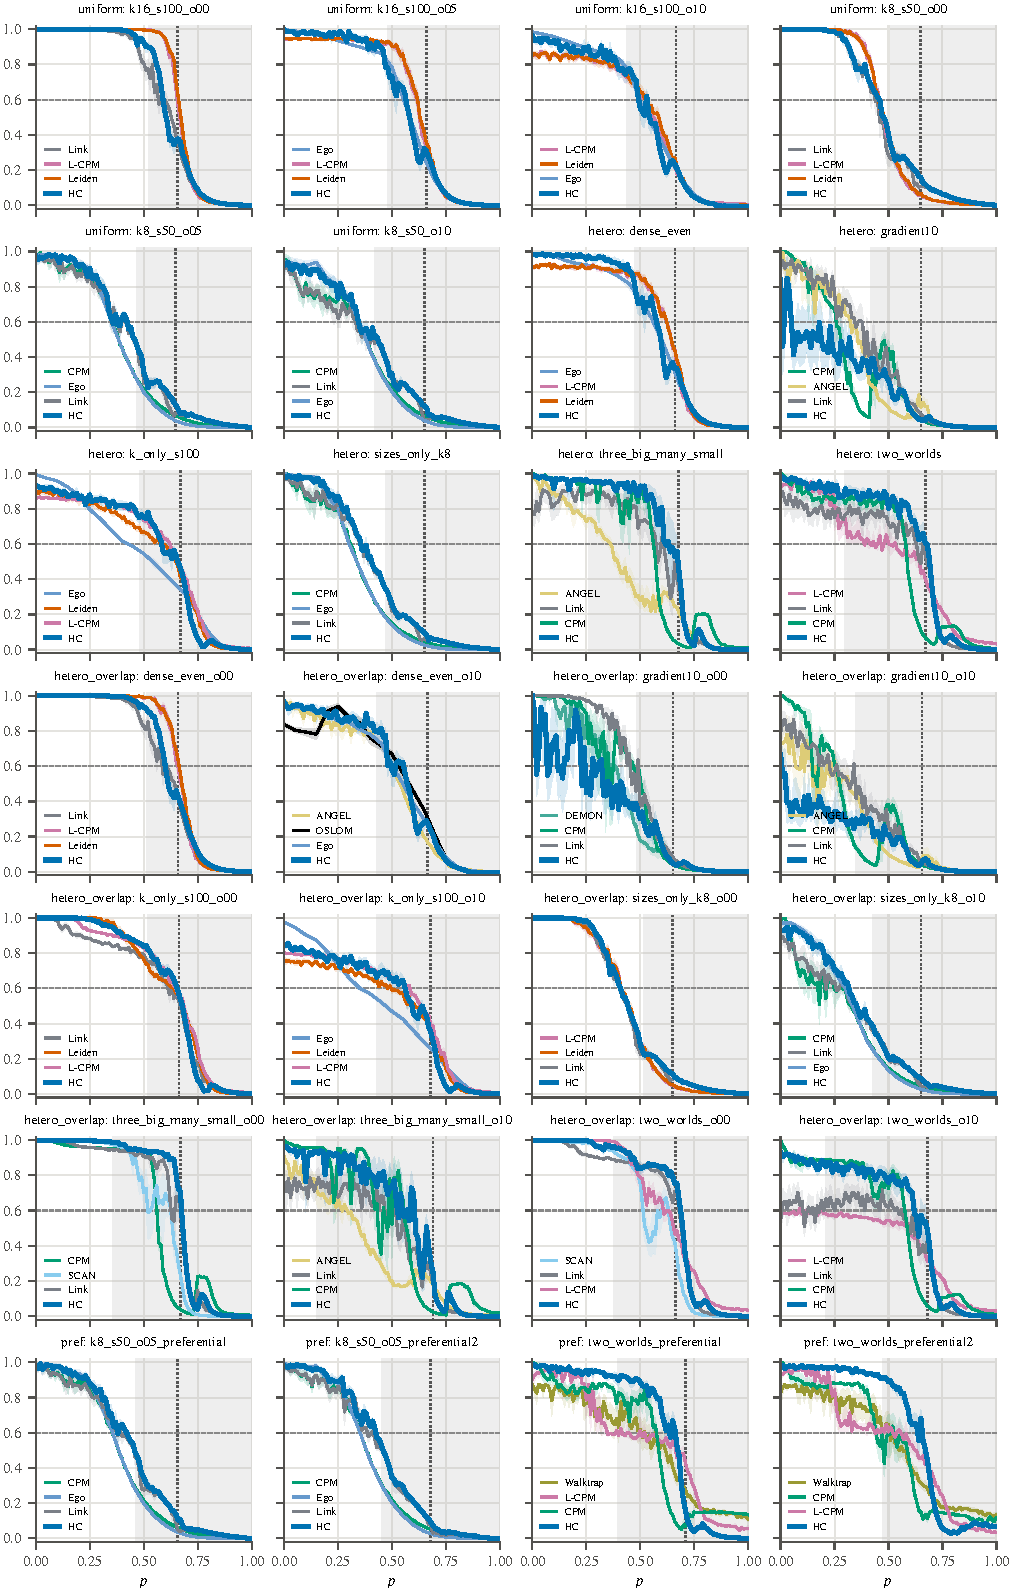
\includegraphics[width=\textwidth]{figures/fig_robust_all.pdf}
  \caption{As Fig.~\ref{fig:robust}, for all 28 ring settings, every parameter chosen
  without labels.}
  \label{fig:S-robust-all}
\end{figure*}

\begin{figure*}[p]
  \centering
  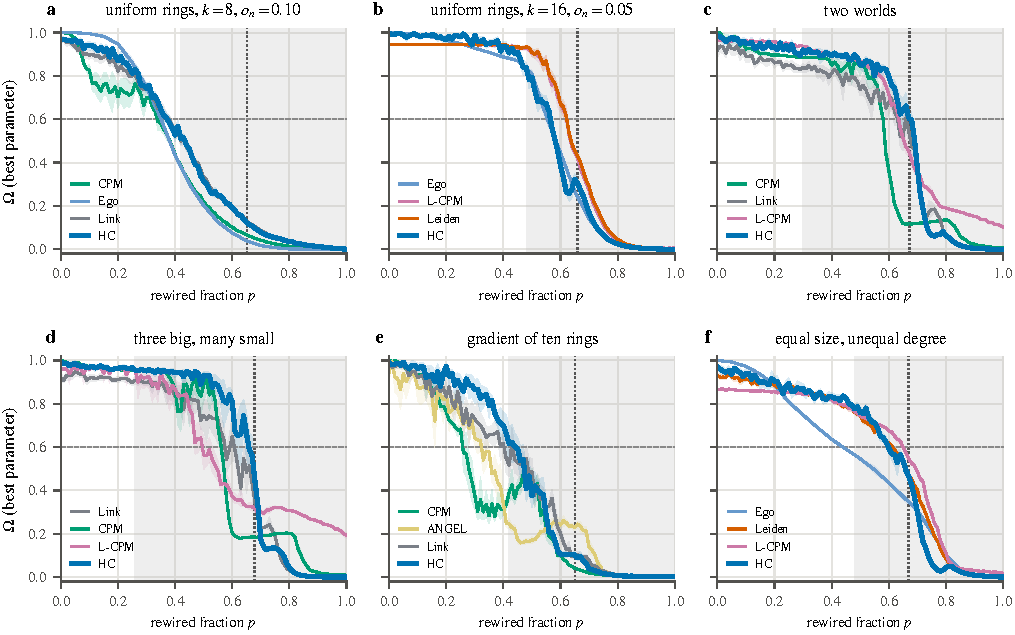
\includegraphics[width=\textwidth]{figures/fig_robust_oracle.pdf}
  \caption{As Fig.~\ref{fig:robust}, with every method at its best parameter on each
  graph (oracle protocol).}
  \label{fig:S-robust-oracle}
\end{figure*}
